
\documentclass{beamer}
\usecolortheme{dove}
\setbeamertemplate{navigation symbols}{}
\usepackage{amsmath,amssymb,amsfonts,amsthm, multicol, subfigure, color}
\usepackage{bm}
\usepackage{graphicx}
\usepackage{tabularx}
\usepackage{booktabs}
\usepackage{hyperref}
\usepackage{pdfpages}
\usepackage{xcolor}
\definecolor{seagreen}{RGB}{46, 139, 87}
\def\independenT#1#2{\mathrel{\rlap{$#1#2$}\mkern2mu{#1#2}}}
\newcommand\indep{\protect\mathpalette{\protect\independenT}{\perp}}
\def\log{\text{log}}
\newcommand\logit{\text{logit}}
\newcommand\iid{\stackrel{\text{iid}}{\sim}}
\newcommand\E{\text{E}}
\newcommand\V{\text{V}}
\renewcommand\P{\text{P}}
\newcommand{\Cov}{\text{Cov}}
\newcommand{\Cor}{\text{Cor}}
\newcommand\doop{\text{do}}
\usepackage{stackrel}
\usepackage{tikz}
\usetikzlibrary{arrows,shapes.arrows,positioning,shapes,patterns,calc}
\newcommand\slideref[1]{\vskip .1cm \tiny \textcolor{gray}{{#1}}}
\newcommand\red[1]{\color{red}#1}
\newcommand\blue[1]{\color{blue}#1}
\newcommand\gray[1]{\color{gray}#1}
\newcommand\seagreen[1]{\color{seagreen}#1}
\newcommand\purple[1]{\color{purple}#1}
\newcommand\orange[1]{\color{orange}#1}
\newcommand\black[1]{\color{black}#1}
\newcommand\white[1]{\color{white}#1}
\newcommand\teal[1]{\color{teal}#1}
\newcommand\magenta[1]{\color{magenta}#1}
\newcommand\Fuchsia[1]{\color{Fuchsia}#1}
\newcommand\BlueGreen[1]{\color{BlueGreen}#1}
\newcommand\bblue[1]{\textcolor{blue}{\textbf{#1}}}
\newcommand\bred[1]{\textcolor{red}{\textbf{#1}}}
\newcommand\bgray[1]{\textcolor{gray}{\textbf{#1}}}
\newcommand\bgreen[1]{\textcolor{seagreen}{\textbf{#1}}}
\newcommand\bref[2]{\href{#1}{\color{blue}{#2}}}
\colorlet{lightgray}{gray!40}
\pgfdeclarelayer{bg}    % declare background layer for tikz
\pgfsetlayers{bg,main} % order layers for tikz
\newcommand\mycite[1]{\begin{scriptsize}\textcolor{darkgray}{(#1)}\end{scriptsize}}
\newcommand{\tcframe}{\frame{
%\small{
\only<1|handout:0>{\tableofcontents}
\only<2|handout:1>{\tableofcontents[currentsection]}}
%}
}

\usepackage[round]{natbib}
\bibliographystyle{humannat-mod}
\setbeamertemplate{enumerate items}[default]
\usepackage{mathtools}

\title{2. The Target Trial}
\author{Ian Lundberg\\Cornell Info 6751: Causal Inference in Observational Settings\\Fall 2022}
\date{25 Aug 2022}

\begin{document}

\maketitle

\section{Feedback \& Logistics}

\begin{frame}{Responding to feedback}
\begin{itemize}[<+->]
\item Questions
\begin{itemize}
\item Are you ok with us asking you to repeat something?
\begin{itemize}
\item Definitely!
\end{itemize}
\item How do I use Calendly?
\begin{itemize}
\item Go to \bref{https://calendly.com/ianlundberg/office-hours}{calendly.com/ianlundberg/office-hours}
\item There are a bunch of time slots. I'm free in all of them.
\item Pick one! You will appear on my calendar!
\end{itemize}
\end{itemize}
\item Suggestions
\begin{itemize}
\item More intuition, examples, then notation
\item Pace was a little fast
\item Those with 0 statistics background found some concepts hard
\item For Cornell Tech, I should repeat questions asked in the room
\item Some confusion about consistency assumption
\item Problem set due Monday, but office hours TTh
\begin{itemize}
\item Ed Discussion
\end{itemize}
\end{itemize}
\end{itemize}
\end{frame}

\begin{frame}{Logistics}
\begin{itemize}
\item Problem Set 1 is due on Monday at 5pm on Canvas
\item We are getting one or more TAs
\end{itemize}
\end{frame}

\section{From Tuesday's reading}

\tcframe

\begin{frame}{Revisit a figure from Tuesday's reading}
\begin{center}
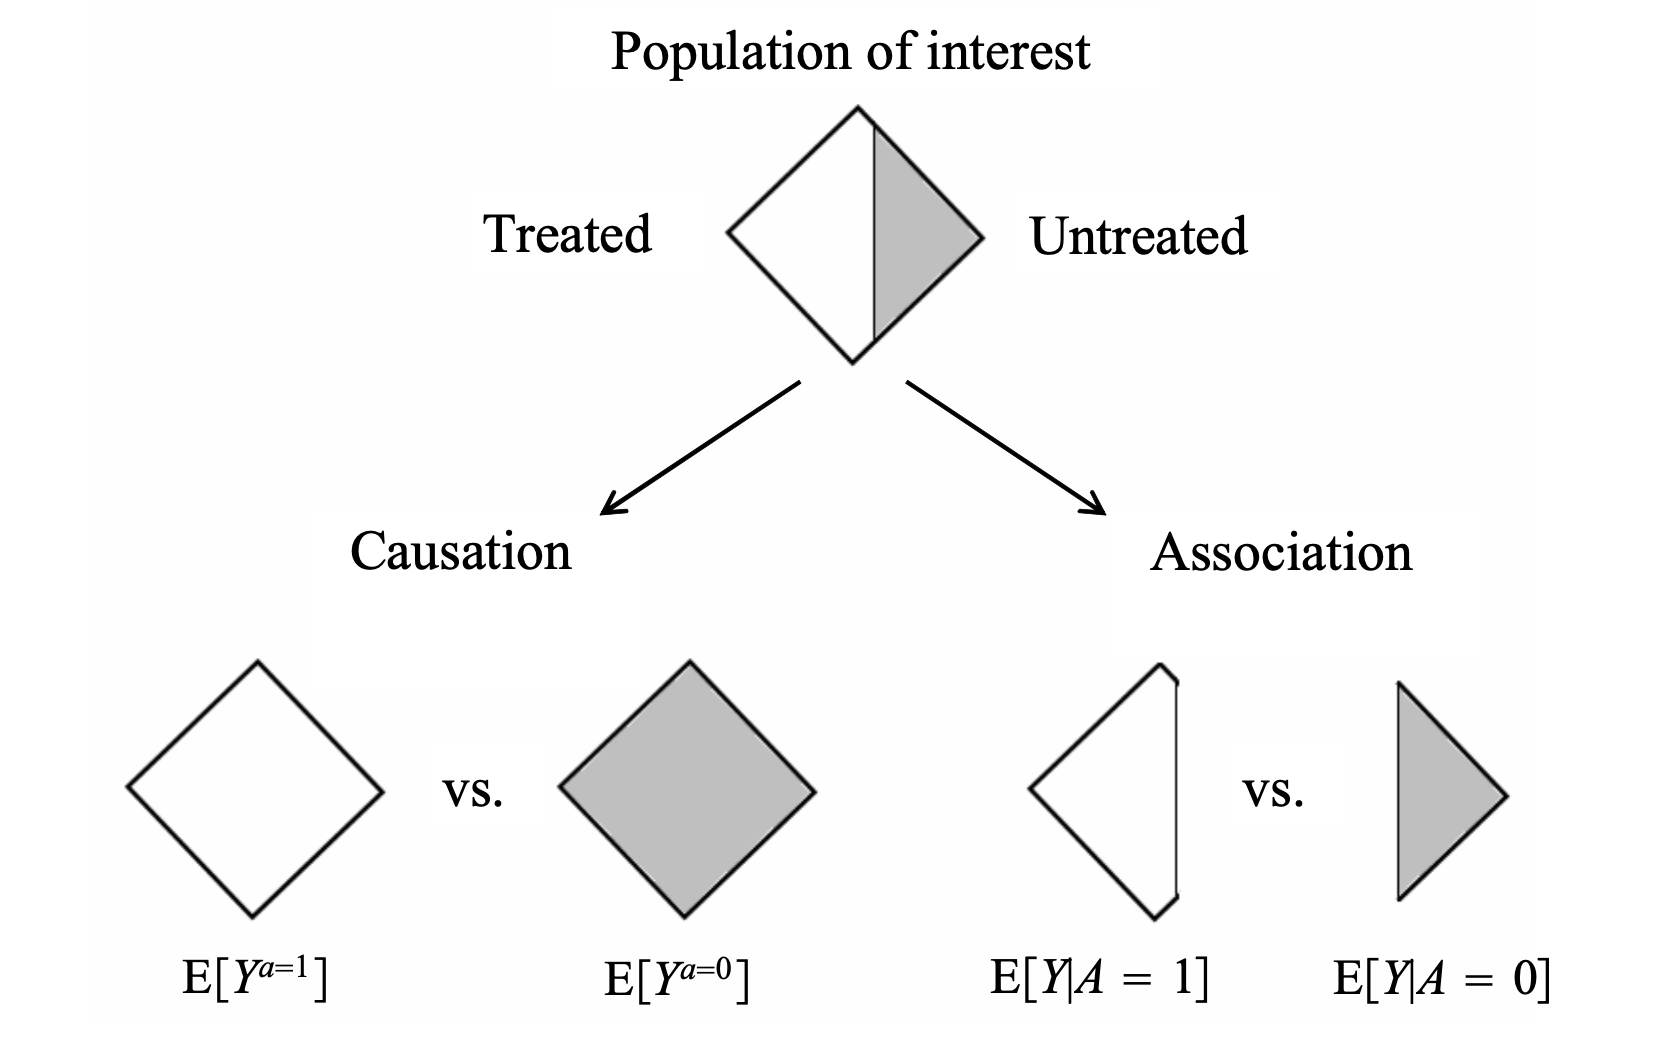
\includegraphics[width = \textwidth]{figures/diamonds} \\ \pause
\end{center}
\textbf{Question}: What if a coin flip assigned units to the white or gray? %\\ \pause
%Then association is causation are the same.
\end{frame}

\section{Randomized experiments: Two key benefits}

\subsection{Exchangeability}

%\tcframe

\begin{frame}
The white and gray are \bblue{exchangeable} \vskip .2in \pause
We will discuss this key idea in three ways:
\begin{itemize}
\item By an experimental procedure
\item By a science table
\item By a mathematical statement of independence
\end{itemize}
\end{frame}

\begin{frame}{\bblue{Exchangeability}: By an experimental procedure}

\begin{tikzpicture}[x = \textwidth, y = \textheight]
%\tikzset{every node}=[font=\small]
\node at (0,0) {};
\node at (1,1) {};
\onslide<2->{
\node[align = center] (coin) at (.5,.9) {Flip a coin\\Two groups of people: heads and tails};
}
\onslide<3->{
\node[align = center] (s1) at (.25, .7) {\bgray{Study 1}\\Heads $\rightarrow$ job training\\Tails $\rightarrow$ no job training};
\draw[->, thick] (coin) -- (s1);
}
\onslide<4->{
\node[align = center] (claim) at (.5, .5) {Compare employment rates\\of those with and without\\job training};
\draw[->, thick] (s1) -- (claim);
}
\onslide<5->{
\node[align = center] (s2) at (.75, .7) {\bgray{Study 2}\\Tails $\rightarrow$ job training\\Heads $\rightarrow$ no job training};
\draw[->, thick] (coin) -- (s2);
\draw[->, thick] (s2) -- (claim);
}
\node<6->[anchor = west, align = left] at (0, .35) {\bgray{Question:} Are both studies valid?};
%\node<7->[anchor = west, align = left] at (0, .22) {Yes. The heads and tails are \bblue{exchangeable}: whether one\\is heads or tails is only related to the outcome\\through the causal effect of job training};
\node<7->[anchor = west, align = left] at (0, .22) {Yes. The (H/T) groups are \bblue{exchangeable}.\\Any statistical pattern between (H/T) and employment\\can only arise from the causal effect of job training};
\end{tikzpicture}

\end{frame}

\begin{frame}{\bblue{Exchangeability}\footnote{See Hern\'an and Robins 2.1}: In a Table}
\begin{itemize}
\item Treatment $A$: Job training or no job training
\item Outcome $Y$: Employed or jobless
\end{itemize}
\vskip .2in
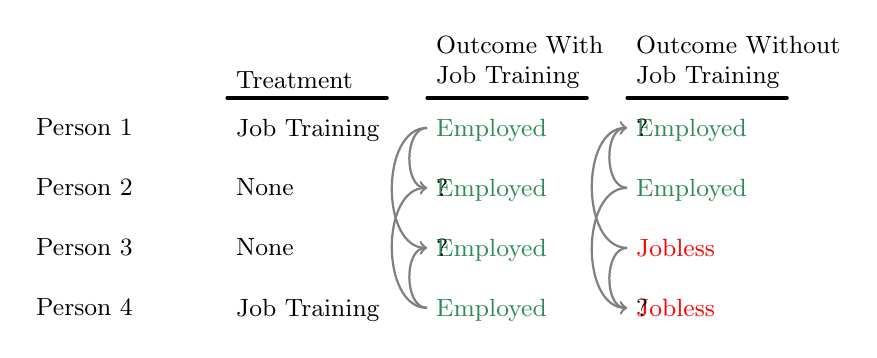
\begin{tikzpicture}[x = 1in, y = .3in]
\tikzset{every node}=[font=\small]
\node[anchor = north west] at (0,-1) {Person 1};
\node[anchor = north west] at (0,-2) {Person 2};
\node[anchor = north west] at (0,-3) {Person 3};
\node[anchor = north west] at (0,-4) {Person 4};
%\onslide<3->{
\node[anchor = south west, align = left] at (2,-.8) {Outcome With\\Job Training};
\node[anchor = south west, align = left] at (3,-.8) {Outcome Without\\Job Training};
\draw[line width = 1.2pt, line cap = round] (2,-.8) -- (2.8, -.8);
\draw[line width = 1.2pt, line cap = round] (3,-.8) -- (3.8, -.8);
\node[anchor = north west] at (2,-1) {\seagreen{Employed}};
\node<1-2>[anchor = north west] at (2,-2) {\seagreen{Employed}};
\node<3->[anchor = north west] at (2,-2) {?};
\node<1-2>[anchor = north west] at (2,-3) {\seagreen{Employed}};
\node<3->[anchor = north west] at (2,-3) {?};
\node[anchor = north west] at (2,-4) {\seagreen{Employed}};
\node<1-2>[anchor = north west] at (3,-1) {\seagreen{Employed}};
\node<3->[anchor = north west] at (3,-1) {?};
\node[anchor = north west] at (3,-2) {\seagreen{Employed}};
\node[anchor = north west] at (3,-3) {\red{Jobless}};
\node<1-2>[anchor = north west] at (3,-4) {\red{Jobless}};
\node<3->[anchor = north west] at (3,-4) {?};
%}
\onslide<2->{
\node[anchor = south west, align = left] at (1,-.8) {Treatment};
\node[anchor = north west] at (1,-1) {Job Training};
\node[anchor = north west] at (1,-2) {None};
\node[anchor = north west] at (1,-3) {None};
\node[anchor = north west] at (1,-4) {Job Training};
\draw[line width = 1.2pt, line cap = round] (1,-.8) -- (1.8, -.8);
}
\onslide<4->{
\draw[->, thick, gray] (2,-1.3) to[out = 180, in = 180] (2,-2.3);
\draw[->, thick, gray] (2,-1.3) to[out = 180, in = 180] (2,-3.3);
\draw[->, thick, gray] (2,-4.3) to[out = 180, in = 180] (2,-2.3);
\draw[->, thick, gray] (2,-4.3) to[out = 180, in = 180] (2,-3.3);
\draw[->, thick, gray] (3,-2.3) to[out = 180, in = 180] (3,-1.3);
\draw[->, thick, gray] (3,-2.3) to[out = 180, in = 180] (3,-4.3);
\draw[->, thick, gray] (3,-3.3) to[out = 180, in = 180] (3,-1.3);
\draw[->, thick, gray] (3,-3.3) to[out = 180, in = 180] (3,-4.3);
}
\end{tikzpicture}
\end{frame}

%\section{Randomized experiment: The gold standard}

\begin{frame}{\bblue{Exchangeability}\footnote{See Hern\'an and Robins 2.1}: In Math}

\begin{itemize} \pause
\item Job training $A$ affects employment $Y$ \pause
\item Statistically, $A$ tells us something about $Y$ \pause
\begin{itemize}
\item Received job training $\rightarrow$ more likely to be employed
\end{itemize} \pause
\item But $A$ tells us nothing about and $Y^{\texttt{Job training}}$
\begin{itemize} \pause
\item Some people would be employed if they received job training \pause
\item Some people would not \pause
\item The coin flip $A$ is unrelated to which kind of person one is
\end{itemize}
\end{itemize} \vskip .2in \pause
In math:
$$A\indep Y^a \qquad\text{for all }a$$
In words:\\
The treatment $A$ is independent\\
of the potential outcomes $Y^a$\\
for all treatment values $a$

\end{frame}

\begin{frame}
\centering \large
Experiments are great because exchangeability holds by design. \vskip .3in \pause
\begin{Large}
But they are also great for other reasons.
\end{Large}
\end{frame}

\subsection{Precise questions}

\begin{frame}

\includegraphics[width = \textwidth]{figures/moderna_begins}\footnote{Published 27 July 2020. \url{https://www.niaid.nih.gov/news-events/phase-3-clinical-trial-investigational-vaccine-covid-19-begins}}
\end{frame}

\begin{frame}{The Moderna trial\footnote{Published 27 July 2020. \url{https://www.niaid.nih.gov/news-events/phase-3-clinical-trial-investigational-vaccine-covid-19-begins}}: What do we like about this design?} \pause
\begin{itemize}
\item ``Trial volunteers will receive two intramuscular injections approximately 28 days apart.'' \pause
\item ``Participants will be randomly assigned 1:1 to receive either two 100 microgram (mcg) injections of mRNA-1273 or two shots of a saline placebo.'' \pause
\item ``The trial is blinded, so the investigators and the participants will not know who is assigned to which group.''
\end{itemize}
\end{frame}

\begin{frame}{The Moderna trial\footnote{Published 27 July 2020. \url{https://www.niaid.nih.gov/news-events/phase-3-clinical-trial-investigational-vaccine-covid-19-begins}}: What do we like about this design?}
\scalebox{.8}{
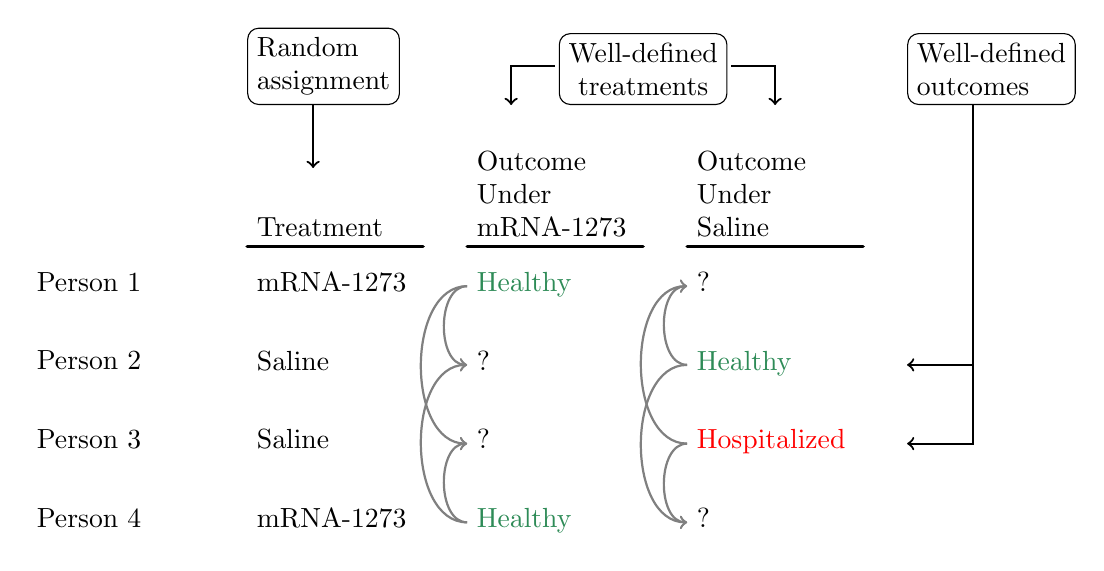
\begin{tikzpicture}[x = 1.1in]
\node[anchor = north west] at (0,-1) {Person 1};
\node[anchor = north west] at (0,-2) {Person 2};
\node[anchor = north west] at (0,-3) {Person 3};
\node[anchor = north west] at (0,-4) {Person 4};
\onslide<2->{
\node[anchor = south west, align = left] at (1,-.8) {Treatment};
\node[anchor = north west] at (1,-1) {mRNA-1273};
\node[anchor = north west] at (1,-2) {Saline};
\node[anchor = north west] at (1,-3) {Saline};
\node[anchor = north west] at (1,-4) {mRNA-1273};
\draw[line width = 1.2pt, line cap = round] (1,-.8) -- (1.8, -.8);
}
\onslide<3->{
\node[anchor = south west, align = left] at (2,-.8) {Outcome\\Under\\mRNA-1273};
\node[anchor = south west, align = left] at (3,-.8) {Outcome\\Under\\Saline};
\draw[line width = 1.2pt, line cap = round] (2,-.8) -- (2.8, -.8);
\draw[line width = 1.2pt, line cap = round] (3,-.8) -- (3.8, -.8);
\node[anchor = north west] at (2,-1) {\seagreen{Healthy}};
\node[anchor = north west] at (2,-2) {?};
\node[anchor = north west] at (2,-3) {?};
\node[anchor = north west] at (2,-4) {\seagreen{Healthy}};
\node[anchor = north west] at (3,-1) {?};
\node[anchor = north west] at (3,-2) {\seagreen{Healthy}};
\node[anchor = north west] at (3,-3) {\red{Hospitalized}};
\node[anchor = north west] at (3,-4) {?};
}
\onslide<4->{
\node[anchor = south, align = center, draw, rounded corners] at (2.8, 1) {Well-defined\\treatments};
\draw[->, thick] (2.4, 1.5) -- (2.2,1.5) -- (2.2, 1);
\draw[->, thick] (3.2, 1.5) -- (3.4, 1.5) -- (3.4, 1);
}
\onslide<5->{
\node[anchor = south west, align = left, draw, rounded corners] at (1,1) {Random\\assignment};
\draw[->, thick] (1.3, 1) -- (1.3, .2);
}
\onslide<6->{
\node[anchor = south west, align = left, draw, rounded corners] at (4,1) {Well-defined\\outcomes};
\draw[->, thick] (4.3, 1) -- (4.3, -2.3) -- (4, -2.3);
\draw[->, thick] (4.3, 1) -- (4.3, -3.3) -- (4, -3.3);
}
\onslide<7->{
\draw[->, thick, gray] (2,-1.3) to[out = 180, in = 180] (2,-2.3);
\draw[->, thick, gray] (2,-1.3) to[out = 180, in = 180] (2,-3.3);
\draw[->, thick, gray] (2,-4.3) to[out = 180, in = 180] (2,-2.3);
\draw[->, thick, gray] (2,-4.3) to[out = 180, in = 180] (2,-3.3);
}
\onslide<8->{
\draw[->, thick, gray] (3,-2.3) to[out = 180, in = 180] (3,-1.3);
\draw[->, thick, gray] (3,-2.3) to[out = 180, in = 180] (3,-4.3);
\draw[->, thick, gray] (3,-3.3) to[out = 180, in = 180] (3,-1.3);
\draw[->, thick, gray] (3,-3.3) to[out = 180, in = 180] (3,-4.3);
}
\end{tikzpicture}
}
\end{frame}

\begin{frame}{The Moderna trial\footnote{Published 27 July 2020. \url{https://www.niaid.nih.gov/news-events/phase-3-clinical-trial-investigational-vaccine-covid-19-begins}}: What do we like about this design?}
\begin{itemize}[<+->]
\item Eligibility criteria clear
\item Blinded
\item Defined follow-up period
\item Well-defined outcome
\item Randomized assignment
\item Pre-registered hypotheses
\end{itemize}
\end{frame}

\begin{frame}

\includegraphics[width = \textwidth]{figures/moderna_end}\footnote{\url{https://www.nih.gov/news-events/news-releases/peer-reviewed-report-moderna-covid-19-vaccine-publishes}}
\end{frame}

\section{Group Exercises}

%\subsection{Design a randomized trial}

\tcframe

\begin{frame}{Part 1) Design a randomized trial}

\Large
This page had links to Google docs for 8 groups to work on the exercise (see exercise on next slides)

\end{frame}

\begin{frame}{Odd numbered groups}
You are a medical researcher focused on high blood pressure. Your research points toward a new drug—MiraclePill—which you believe will cause lower blood pressure in patients who are at risk (you are the expert, so you can define this). You aren’t sure of the correct dosage: you think somewhere between 0 and 100 mg per week. \vskip .2in

How would you design a randomized trial to assess MiraclePill? \vskip .2in

\begin{enumerate}
\item What is the intervention?
\item What is the outcome?
\item What is the follow-up period between treatment and outcome?
\item Who is the target population?
\item How are unit-level quantities aggregated to a population-level summary?
\end{enumerate}

\end{frame}

\begin{frame}{Even numbered groups}
You are a social scientist focused on the underrepresentation of women in computer science at the BA level. You develop a new mentorship program to connect entering first-year women computer science majors with recent women Cornell alumni from CS. The alumni agree to meet one-on-one with the first-year undergraduates a couple times a year. You want to randomize some element of this program in order to test its effectiveness. \vskip .2in

How would you design a randomized trial to assess the mentorship program? \vskip .2in

\begin{enumerate}
\item What is the intervention?
\item What is the outcome?
\item What is the follow-up period between treatment and outcome?
\item Who is the target population?
\item How are unit-level quantities aggregated to a population-level summary?
\end{enumerate}

\end{frame}

%\subsection{Compare to observational evidence}

\begin{frame}
\huge Observational evidence \vskip .2in
Scroll down to Part 2
\end{frame}

\begin{frame}{Odd numbered groups}

Another medical researcher comes to you with observational evidence. ``I had 100 people in my office today. 50 of them tell me they take MiraclePill 100mg once per week. The other 50 tell me they do not take MiraclePill. Average blood pressure was lower for those who take MiraclePill.'' \vskip .2in

What do you say to this researcher? How is their evidence different from your target trial?

\end{frame}

\begin{frame}{Even numbered groups}

Another social scientist comes to you with observational evidence. ``Today I was at a gathering of women Cornell alumni from the CS and English departments. I went around and asked them if they ever engaged with CS alumni during college. 75\% of the CS graduates said yes, but only 10\% of the English graduates said yes. I think engaging with alumni is key to persistence in CS.'' \vskip .2in

What do you say to this researcher? How is their evidence different from your target trial?

\end{frame}

%\subsection{A hypothetical target trial for an observational claim}

\begin{frame}

\huge Hypothetical target trial \vskip .2in
Scroll down to Part 3

\end{frame}

\begin{frame}{Odd numbered groups}

A researcher (with whom you may disagree) says to you: “Coming to office hours frequently causes student success in the classroom.” \vskip .2in

Your task is to create the details that would make this observational claim specific. 
What is the target trial?  \vskip .2in

\begin{enumerate}
\item What is the hypothetical intervention?
\item What is the outcome?
\item What is the follow-up period between treatment and outcome?
\item Who is the target population?
\item How are unit-level quantities aggregated to a population-level summary?
\end{enumerate}

\end{frame}

\begin{frame}{Even numbered groups}

A researcher (with whom you may disagree) says to you: “Single parenthood causes poverty. If poor women would marry, then they would no longer be poor.”  \vskip .2in

Your task is to create the details that would make this observational claim specific. 
What is the target trial?  \vskip .2in

\begin{enumerate}
\item What is the hypothetical intervention?
\item What is the outcome?
\item What is the follow-up period between treatment and outcome?
\item Who is the target population?
\item How are unit-level quantities aggregated to a population-level summary?
\end{enumerate}

\end{frame}

\section{General discussion}

% I AM HERE

\tcframe

\begin{frame}
In an observational study, you cannot randomize. \pause \vskip .2in
But you can do all the other things\footnote{Hern\'an, M. A., \& Robins, J. M. (2016). Using big data to emulate a target trial when a randomized trial is not available. American Journal of Epidemiology, 183(8), 758-764.} \pause
\begin{itemize}
\item Eligibility criteria \pause
\item Treatment strategies \pause
\item Assignment procedures (to discuss more Sep 6) \pause
\item Follow-up period \pause
\item Outcome \pause
\item Causal contrasts of interest \pause
\item Analysis plan
\end{itemize}
\end{frame}

\begin{frame}{Let me know what you are thinking}

\begin{huge} \bref{https://tinyurl.com/CausalQuestions}{tinyurl.com/CausalQuestions} \end{huge}
\vskip .7in

Office hours TTh 11am-12pm and at \bref{https://calendly.com/ianlundberg/office-hours}{calendly.com/ianlundberg/office-hours}\\Come say hi!

\end{frame}


\end{document}


